\section*{}
\begin{center}
    {\fontsize{14}{1.5}\selectfont \textbf{CHAPTER III}}\\
    \vspace{12pt}
    {\fontsize{16}{1.5}\selectfont \textbf{Methodology}}\\
    \vspace{12pt}
    \vspace{12pt}
\end{center}

\setcounter{section}{3}
\setcounter{subsection}{0}
\addcontentsline{toc}{section}{\textbf{CHAPTER III Methodology}} % Add to ToC

\renewcommand{\theequation}{\thesection.\arabic{equation}}
\renewcommand{\thetable}{\thesection.\arabic{table}}
\renewcommand{\thefigure}{\thesection.\arabic{figure}}
\setcounter{table}{0}
\setcounter{figure}{0}
\setcounter{equation}{0}
\setlength{\parindent}{0pt}






% \subsection{Detailed Methodology} {
% \begin{figure}[hbt!]
%     \centering
%     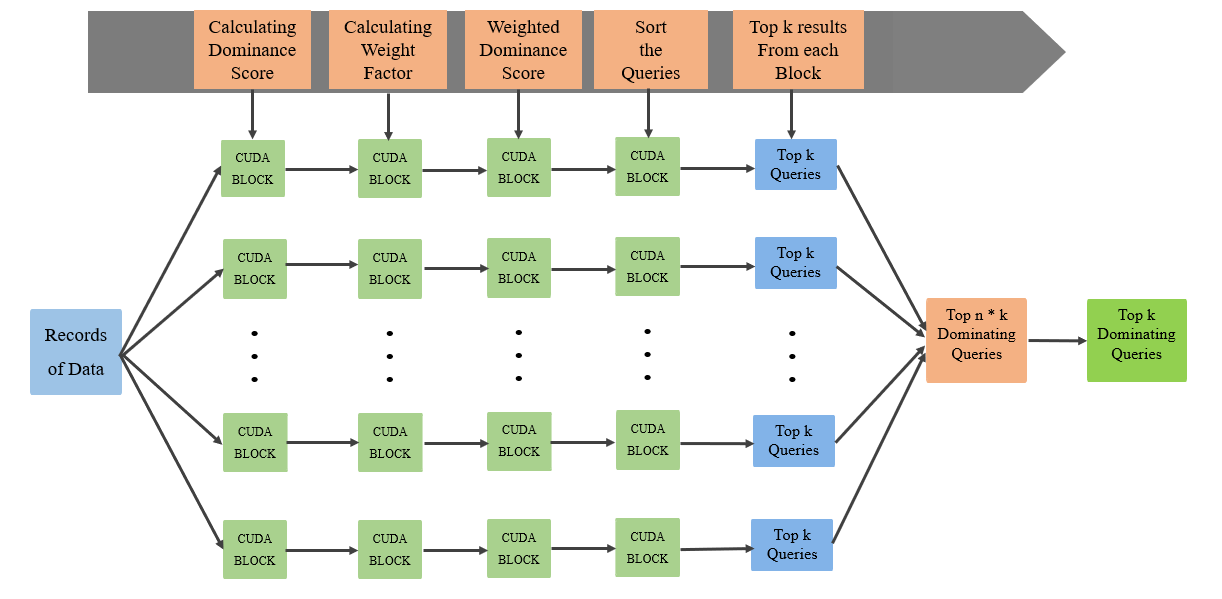
\includegraphics[width=\textwidth, height=9cm]{img/architecture.png}
%     \caption{Proposed architecture}
%     \label{fig:proposed_architecture}
% \end{figure}
% % The entire record of data is divided into n number of blocks and each block contains m number of threads.
% % Each block calculates the Dominance Score, Weight Factor, Weighted Dominance Factor of their respective records independently of each other. After Weighted dominance score is calculated the records are sorted based on their score and top-k records from each block is retrieved. If there are n number of such blocks, top n * k records are found. Then, from those records top-k records could be retrieved using brute force or any other technique.\\
% The data record is divided into multiple blocks, with each block containing a set number of threads. Within each block, calculations are performed independently to determine the Dominance Score, Weight Factor, and Weighted Dominance Factor for the respective records. Once the Weighted Dominance Score is computed, the records are sorted based on their scores, and the top-k records from each block are extracted.

% If there are multiple blocks (n in total), the process is repeated for each block, resulting in the identification of a combined set of top records (n * k records). Finally, from this combined set, the top-k records are retrieved using either brute force or other relevant techniques. This procedure allows for the efficient identification of the most significant records across the entire dataset.

\subsection{Methodology}
{
\subsection{"E2E-LOAD: End-to-End Long-form Online Action Detection," ICCV 2023}

Data Preparation:

The dataset contains long videos with action labels. The frames are processed to extract spatial and temporal features from a backbone neural network. The extracted feature points are saved in a Stream Buffer (SB) so as to successfully operate incoming video frames.

Model Architecture:

Short-term Modeling:

Using Stream Buffer, the method captures spatial characteristics within parts of video frames.

For this reason spatiotemporal modeling is needed to understand short-term dependencies.

The design of ‘Space-then-Space-time’ helps to handle well the representational capacity of anything more than that it is also efficient enough for taking care of those cases where there has been an increase in the loading time leading into a large amount of data being received than before.

Spatiotemporal interactions among most recent chunks of frames are created by multi-layer attentions.

Causal mask ensures that no future frame information leaks into current frame prediction.



To cover longer temporal contexts, they compress long historical sequences of frames.

In order to achieve computational efficiency, compression module uses spatiotemporal attention with greater down-sampling rate.

These long term sequences are detached so as to avoid back propagation making training complicated and focused gradient updates on SB only.

Training:

Education on any part or all element


\subsection{ "Learning to Discriminate Information for Online Action Detection," CVPR 2020
}

Data Preparation:

The dataset preparation involved the use of TVSeries and THUMOS-14 which contained untrimmed videos with temporal annotations for different actions. Every frame was annotated and processed so as to extract action detection relevant features.

Model Architecture:

Information Discrimination Unit (IDU):

IDU works on video frames through a fully connected layer to extract hidden states that enable probability distribution over ongoing actions.

These distributions are then passed through a softmax function for classification purposes.

Loss Function:

Cross entropy loss is used to define the classification loss (La).

Loss function L combines together classification loss La, feature extraction loss Le and consistency loss Lc in a multi-task manner.

Training:

During training, the model’s multi-task loss function is minimized by adjusting parameters to make it strike equilibrium between action classification accuracy and feature consistency.

Evaluation:

Mean average precision (mAP) and mean calibrated average precision (mcAP) were used to evaluate the performance of the model.

mAP measures the average precision across all frames for each action class whereas mcAP compensates for positive-to-negative ratio of frames thus addressing class imbalance issues.

Ablation Studies:


\subsection{ A novel online action detection framework from untrimmed video
streams}

Data Preparation:

The dataset entails several videos labeled for actions taken in them.A neural network is applied to processed video frames to get out necessary features for action detection.

Model Architecture:

Feature Extraction:

Spatial and temporal features on the other hand are extracted from video frames by use of a deep convolutional neural network.

These features essentially make the model holistic enough to understand what happens in a given video clip.

Sequence Modeling:

And recurrent neural networks or transformers are used respectively to capture the temporal relations between frames.

Atteniton mechanism is introduced where related parts of these sequences can be inspected more closely and thus boosting its performance on detecting actions within them with higher precision.

Training

The training process involves minimization of a loss function which combines classification accuracy and temporal consistency of an LSTM based RNN model used by us for action recognition.

This means that techniques like BPTT (back-propagation through time) are adopted here so that this model might have its parameters optimized to learn the temporal dynamics of actions associated with it hence enabling it differentiate between different types of such movement-based activities.

Evaluation:

To assess the performance, the model is tested using standard metrics such as accuracy, precision, recall and F1 score on benchmark datasets.Metrics, indicating how efficient our approach was in detection tasks were compared to other existing works.

Additional Techniques:

Methods for data augmentation
}


\begin{figure}[htbp]
    \centering
    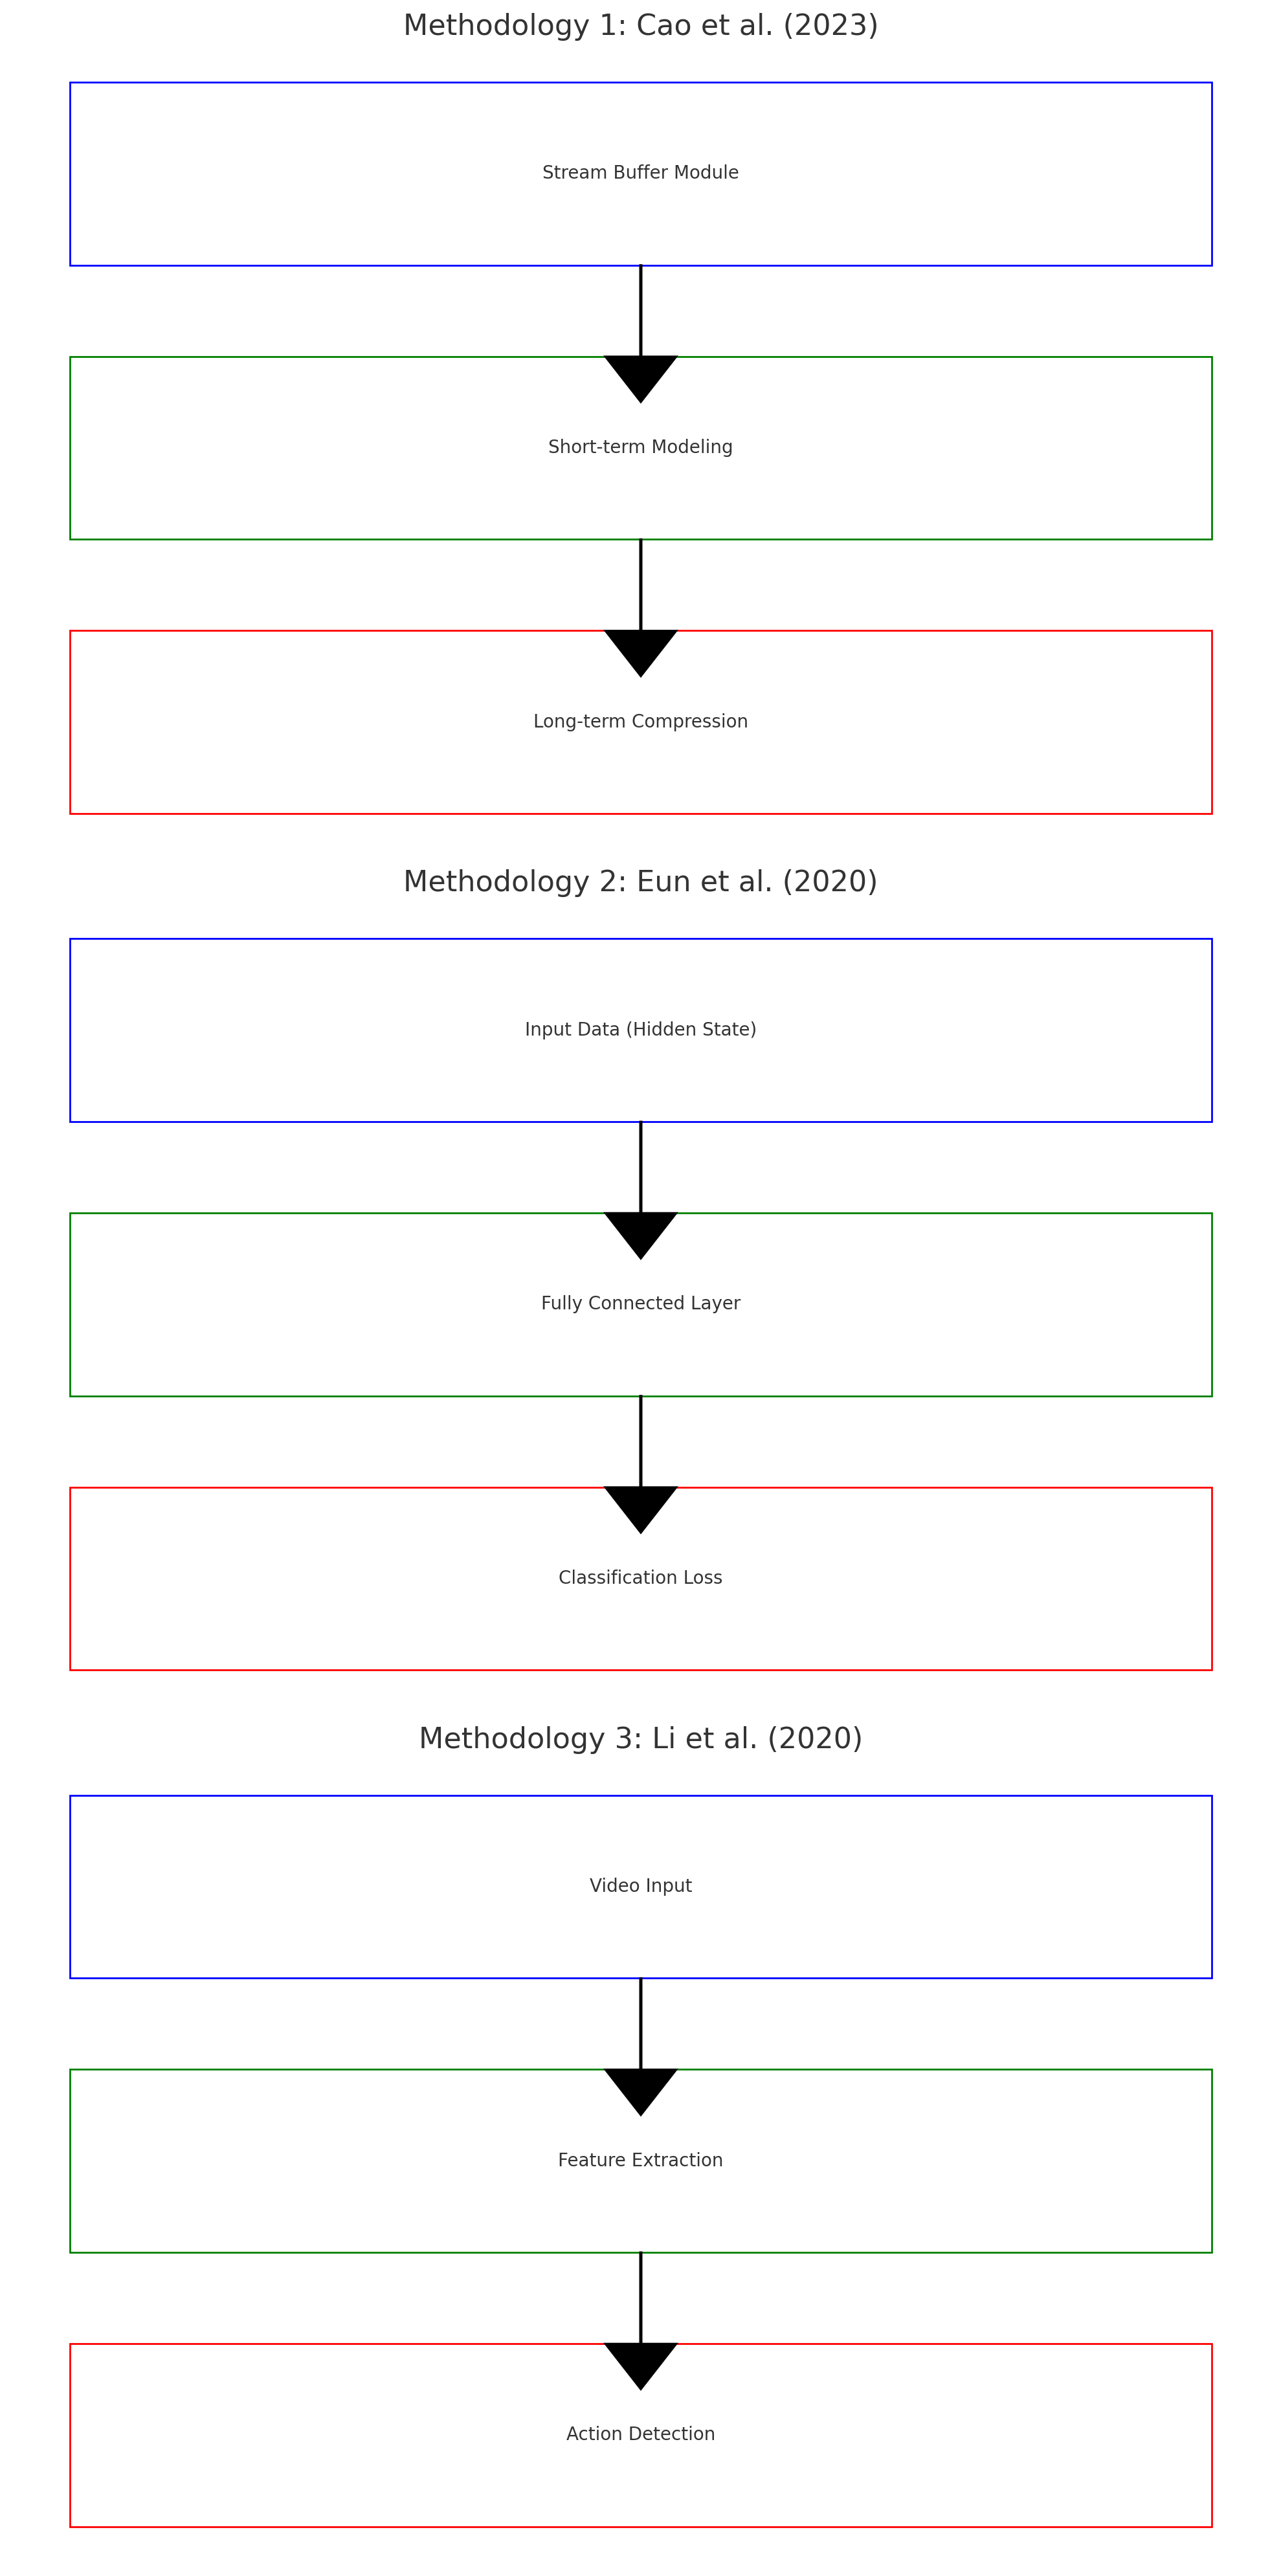
\includegraphics[width=4.5in]{img/method.png}
    \caption{Proposed Methodology}
    \label{fig:example}
\end{figure}




